% Koma class
\documentclass[a4paper, oneside]{scrartcl}   

\usepackage{a4wide}

%------------------
% language = english
\usepackage[english, german]{babel}	% Umlaute mit \"u
\usepackage[latin1]{inputenc}

% margins + Kopf- und Fu�zeilen
\usepackage[left = 2.5cm, right = 2.5cm, top = 2cm, bottom = 3cm]{geometry}
\usepackage{scrpage2} 
\pagestyle{scrheadings}
\clearscrheadfoot
\rehead{\headmark}
\lehead{\pagemark}
\lohead{\headmark}
\rohead{\pagemark} 


% math
\usepackage{amssymb}
\usepackage{amsmath}

% figures
\usepackage{tikz}
\usepackage{graphicx}


% section-Zaehler wird neu gesetzt:
\setcounter{section}{2}
%------------------
\author{Sascha Meiers, Martin Seeger}
\title{Exercise 2, Discrete Mathematics for Bioinformatics}
\date{Winter term 2011/2012}


\begin{document}
\maketitle

%---------------------------------------------------------------------------------------------------

\subsection{Modulo Arithmetic}

\noindent a) We show that $\langle a \rangle \subset \langle d \rangle$.

Since $d = \mathrm{gcd}(a, n)$, there is a $k \in \mathbb{N}$ such that $a = kd$.
Hence, if $v \in \langle a \rangle$, i.e. $v = ai \mod n$, then $v = dki \mod n$ which implies that $v \in \langle d \rangle$.
\\

\noindent b) We show that $\langle a \rangle \supset \langle d \rangle$.

Any element $v$ of $\langle d \rangle$ can be written as $v = di\mod n$ (*).
On the other hand, $v \in \langle a \rangle$ iff $v = aj\mod n$.

We now use Bezout's lemma to find $x$, $y$, such that $ax + ny = d$. This is inserted into (*) to yield
\[
v = di\mod n = (ax + ny)i\mod n = axi\mod n.
\]
In other words, $v \in \langle a \rangle$. $\square$
\\

\subsection{Hashing}

Let $x,y$ be character strings both of length $n$. Now we can interprete their characters 
as numbers in radix $2^p$, leading to a hash function 
\[h(x) = \sum\limits_{i=0}^n x_i 2^{p\cdot i} \text{ mod } 2^p-1\]
If $y$ is nothing else than a permutation of the characters in $x$, 
then especially their sum of the digits is equal, i.e.
\[ \sum\limits_{i=0}^n x_i = \sum\limits_{i=0}^n y_i  \]
Proof: $h(x) = h(y)$
\begin{align}
h(x) &= \sum\limits_{i=0}^n x_i 2^{p\cdot i} \text{ mod } 2^p-1  \\
     &= \sum\limits_{i=0}^n \left( x_i 2^{p\cdot i} \text{ mod } 2^p-1 \right) \text{ mod } 2^p-1  \\
     &= \sum\limits_{i=0}^n \left( x_i \text{ mod } 2^p-1 \right) \left( \underbrace{2^p \text{ mod } 2^p-1}_1 \right)^i \text{ mod } 2^p-1 \\
     &= \sum\limits_{i=0}^n x_i \text{ mod } 2^p-1  \\
     &= \sum\limits_{i=0}^n y_i \text{ mod } 2^p-1  \\
     &= h(y)
\end{align}


\subsection{Hashing}

We choose two different hash functions $h_1$ and $h_2$ and simulate hashing with chaining for random integer variables. 
We take a fixed table size of $ p = 48049$, which is a prime number, 
and analyze the distribution of the inserted elements in the hash table.
Therefore we measure the maximum chain length as well as the standard deviation of the chains' lengths 
for load factors from zero up to ten.
The average chain length is equal to the load factor. 
The figures show the measured values for both hash functions
\[h_1(x) = x \text{ mod } p \qquad h_2(x) = p \left( \frac{\sqrt{5}-1}{2} x \text{ mod } 1 \right)  \]

\begin{centering}
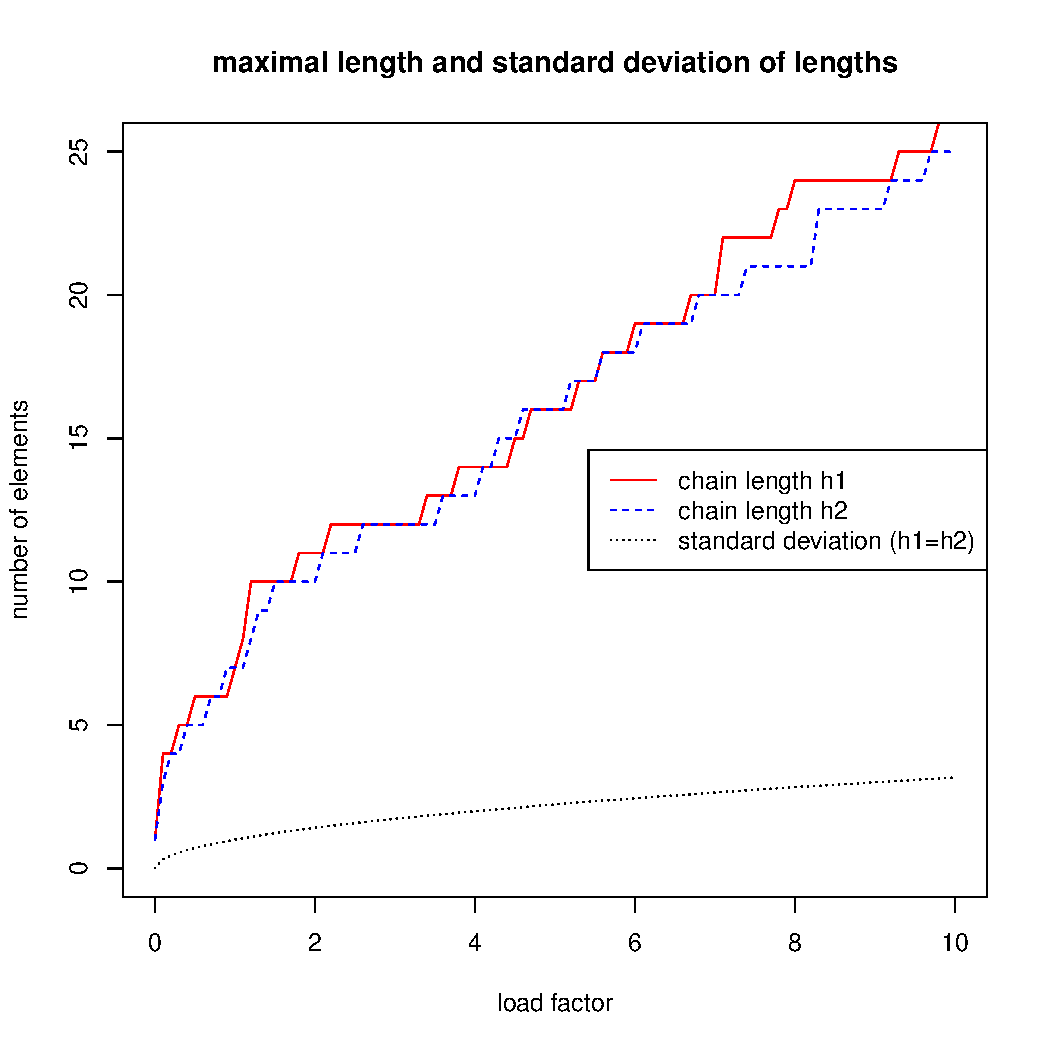
\includegraphics[width=\textwidth] {plot}
\end{centering}

Obviously both hash functions distribute both with nearly the same quality. The maximum length is usually 
more than twice as large as the load factor, which is the lower bound. Of course these results mainly 
depend on the input data, which here comes from Python's random command (uniformely distributed numbers $\in \{0,.., 2^{20} \}$ )

\subsection{Expected value}



\end{document}
